\section{Introduction}\label{section:intro}
Experimental design is a systematic approach to specifying every
possible aspect of an experiment \cite{chaloner1995}. In this study,
we focus on experiments that involve measuring quantities arising from
naturally occurring processes. For us, therefore, experimental design
entails determining which specific measurements to record from a given
process. In a typical experiment the number of measurements that can
be recorded is limited by time, cost and other constraints. Therefore
selecting the right set of measurements to record is crucial as it
directly impacts the utility of the data collected, and consequently,
the validity of the conclusions drawn.

For example, consider the process of searching for oil: measurements
require digging deep holes in the ground, known as "boreholes". A
\emph{design} simply indicates which boreholes should be dug
\cite{horesh2008borehole}. Since digging boreholes is expensive, only
a limited number of them can be dug, and thus carefully choosing their
locations is crucial.

Specifying the right set of measurements holds particular significance
when solving an \emph{inverse problem} --- i.e.~making inference of
the physical world utilizing a physical model of a phenomenon of
interest \cite{tarantola2005,kaipio2005}. In an inverse problem, we
seek to infer physical quantities, based on observations and a model
of the physical world. Models are typically phrased in the language of
ordinary or partial differential equations.

Inverse problems are ubiquitous in science and engineering. For
example, in electrical impedance tomography (EIT) we seek to infer the
structure of the inside of a human body. Inference is conducted based
on observations of electrical current impedance measured at specific
electrode locations on the skin, leveraging known equations of
electric current flow \cite{horesh2010impedance}. Magnetic Resonance
Imaging (MRI) also entails solving an inverse problem. There,
radio-frequency pulses are sent through the human body in the presence
of a strong magnetic field. The response of one's body contents to
these radio-frequency pulses is measured, allowing a radiologist to
view the internals of a body in a noninvasive manner
\cite{horesh2008mri}. An inverse problem also arises in oil and gas
exploration, where acoustic waves are sent through "boreholes" ---
deep cylindrical wells drilled into the ground. Data of travel and
return times of the acoustic waves are recorded. Wave travel and
return time is influenced by the properties of the subsurface
materials, such as density, elasticity, and the presence of fluids or
voids. Combining travel time data with a geophysical model of the
contents of the earth's crust facilitates reconstructing the structure
of the subsurface in a process called \emph{borehole tomography}
\cite{horesh2008borehole}. Inverse problems also arise in many other
areas of seismology and geology \cite{rabinowitz1990, steinberg1995}
and medical imaging \cite{tarantola2005}. In many inverse problems the
goal is to infer some numerical parameter. However, in the formulation
we consider in this study, as well as in the examples above, the goal
is to conduct inference over some \emph{function} over $\Omega$, where
\(\Omega \subseteq \mathbb{R}^d, d=1,2,3\) is a spatial domain of
interest.

\subsection{D-optimal Designs}\label{subsec:D}
In all of the examples of inverse problems we have seen, as well as in
many other applications, only a limited number of measurements are
allowed. For example, in borehole tomography, a measurement involves
drilling a deep well in the ground --- a very costly endeavor. In
medical imaging applications like MRI, the time allotted for each
patient in the MRI machine limits the number of measurements that can
be taken during a single session. Therefore, measurements should be
chosen to extract as much information from the experiment. Typically,
a user will consider some utility, called a \emph{design criterion}
and take measurements that maximize this utility. Two of the most
widely recognized and extensively studied design criteria are the A-
and \emph{D-optimality} criteria.

In this study, we focus on the Bayesian D-optimality
criterion. Bayesian D-optimality carries a simple and intuitive
meaning: measurements chosen according to the D-optimality criterion
maximize the expected Kullback-Leibler (KL) divergence from posterior
to prior \cite{chaloner1995, AlexanderianGloorGhattas14,
  CoverThomas91}.
%%  Utilizing KL divergence for quantifying differences between
%% distributions is standard practice and we will not motivate it
%% further here.
Recall that for a discrete parameter $\param$ and data $\data$, the KL
divergence is defined as
\begin{equation}\label{eq:basic_KL}
  D_{KL}\left (\Pr(\param|\data)||\Pr(\param)\right ) =  \sum_{\param} \log
  \frac{\Pr(\param|\data)}{\Pr(\param)} \Pr(\param|\data). 
\end{equation}
Of course, data $\data$ is not known before the experiment is
conducted. Hence, we average over $\data$ to define the D-optimality
criterion as:
\begin{equation*}
  \mathbb{E}_{\data}\left [ D_{KL}\left (\Pr(\param|\data)||\Pr(\param)\right ) \right ].
\end{equation*}
We refer to a set of measurements that maximizes the D-optimality
criterion as a \emph{D-optimal design}.

For a linear model with Gaussian prior in finite dimensions, a
D-optimal design minimizes the determinant of the posterior covariance
\cite{chaloner1995}. In Section \ref{subsec:D_optimal_design} we give
a more general definition of the D-optimality criterion that applies
to arbitrary measures. We also show how the D-optimality criterion
generalizes to linear models over infinite-dimensional Hilbert spaces
(e.g.~function spaces).

\subsection{A toy model: the 1D heat equation}\label{subsec:toy}
For concreteness, let us now consider a toy inverse problem: inferring
the initial condition for a partial differential equation known as the
\emph{heat equation} in one dimension (1D heat equation
henceforth). Readers less familiar with partial differential equations
can think of the following setup: before us there is a metal rod,
perfectly insulated except for its tips. At each point on the rod the
temperature is different and unknown, and we call this temperature
distribution the \emph{initial condition}. We wait for a short time
$T$ and let the heat dissipate a bit inside the rod. The heat equation
determines the heat distribution inside the rod at time $t=T$.

The full time evolution of heat in the rod $\Omega=[0,1]$ is formally
described by the following three equations:
\begin{subequations}
  \begin{alignat}{2}
    u_t &= \Delta u &&\qquad \text{in } [0,1] \times [0,\infty), \label{eq:heat1}\\
    u &= 0 &&\qquad \text{on } \{0, 1\} \times [0,\infty), \label{eq:heat2}\\
    u &= u_0 &&\qquad \text{on }[0,1] \times \{0\}. \label{eq:heat3}
  \end{alignat}
\end{subequations}
As time passes, heat dissipates across the rod as hotter regions,
e.g.~local maxima of the heat distribution, become cooler. This
behavior is captured by eq.~\eqref{eq:heat1}: the Laplacian at local
maxima is negative, so $u_t = \Delta u$ implies $u$ decreases at its
maxima, and the reverse happens at local minima. Eq.~\eqref{eq:heat2}
describes the \emph{boundary condition}, which dictates how heat
interacts with the outside world at the two edges of the rod
$\{0,1\}$. Specifically, eq.~\eqref{eq:heat2} implements an absorbing
boundary, i.e.~heat that interacts with the boundary immediately
disappears. This type of boundary condition is known as a
\emph{homogeneous Dirichlet boundary condition}. Eq.~\eqref{eq:heat3}
describes the \emph{initial condition}, i.e.~the heat distribution
inside the rod at time $t=0$.

Solving the 1D heat equation is straightforward. Consider an initial
heat distribution $u_0\in L^2([0,1])$ that satisfies the homogeneous
Dirichlet boundary condition eq.~\eqref{eq:heat2}. This initial
condition $u_0$ is a linear combination of sines $\ev_n(x) = \sin(\pi
n x)$, so $u_0 = \sum_{n\geq 1} a_n \ev_n$ for some $\{a_n\}_{n\geq
  1}$. Now, note that $\ev_n$ are in fact eigenvectors of the
Laplacian: $\Delta \ev_n = -\pi^2 n^2\ev_n$. It should not be hard to
believe that $u(\cdot, T) = \sum_{n\geq 1} a_n \exp(-\pi^2 n^2T )
\ev_n$ \cite{renardy2006PDE}. Thus, eigenvectors of the linear
operator that describes the time evolution of heat are $\ev_n(x) =
\sin(\pi n x)$ with corresponding eigenvalues
\begin{equation}\label{eq:decay}
  \exp(-\pi^2 n^2T ).
\end{equation}

In the \emph{inverse problem of the 1D heat equation}, our goal is to
infer the initial condition $u_0 = u(\cdot, 0)$ from noisy
observations of the final state $u(\cdot, T)$. However, we are not
able to measure $u(\cdot, T)$ at every point in the domain
$\Omega$. Rather, we take some number of temperature measurements on
the rod once our waiting time $T$ has passed and try to infer
$u(\cdot, 0)$ from these measurements.

The inverse problem of the 1D heat equation is difficult ("ill-posed")
since heat spreads in a diffusive manner and any roughness in the
initial condition is quickly smoothed, as implied by the squared
exponential decay of eigenvalues in eq.~\eqref{eq:decay} with
$n\to\infty$. See Supplementary movies S1 and S2 for an illustration
of this phenomenon\footnote{Code generating these movies is located in
module \texttt{movies.py} in the accompanying
\href{https://github.com/yairdaon/OED}{repository}.}. For ill-posed
problems regularization is required, and we implement such
regularization via a fully Bayesian formulation of the inverse
problem.


In order to find a fully Bayesian formulation for our inverse problem
we first need to specify a prior on \emph{functions} defined over
$\Omega = [0,1]$. For the sake of simplicity we would like to utilize
a Gaussian prior. While specifying the prior mean is easy --- we take
the zero function on $\Omega$ --- specifying a prior covariance is
more involved. In analogy with the finite dimensional case, we seek a
covariance \emph{operator} that is positive definite and imposes
sufficient regularity on functions over $\Omega$. Thus, we set our
prior for the initial condition $u_0 \sim \mathcal{N}(0,
(-\Delta)^{-1})$, where $\Delta$ is again defined with a homogeneous
Dirichlet boundary condition. The intuition here is that since
$\Delta$ is a differential operator, it is "roughing" (the opposite of
smoothing) and so $(-\Delta)^{-1}$ is smoothing. Prior realizations
are generated, in analogy to the finite dimensional case, by smoothing
white noise: $(-\Delta)^{-1/2}\mathcal{W}$, where $\mathcal{W}$ is
white noise \cite{rue2011}. Our choice of prior covariance operator
ensures the posterior is well-defined and prior realizations are
well-behaved, see Theorem 3.1 and Lemma 6.25 in \cite{Stuart10} for
details. The second ingredient of a fully Bayesian formulation of the
inverse problem is likelihood. We simply assume centered iid Gaussian
measurement error model, giving rise to a the widely applicable
Gaussian likelihood function.

Now that we have a fully Bayesian formulation of our toy inverse
problem, we would like to find a D-optimal design. Defining D-optimal
designs over function spaces is somewhat mathematically
involved. Thus, to keep our discussion here focused, we will explore
these technical details later in Section
\ref{subsec:D_optimal_design}. For now, it suffices to know that
D-optimal designs can be defined for our problem.


\subsection{Measurement Clusterization}
Surprisingly, A- and D-optimal designs for inverse problems have been
observed to yield remarkably similar measurements in certain cases
\cite{fedorov1996, nyberg2012, fedorov1997, Ucinski05,
  neitzel2019sparse}. This phenomenon is illustrated for our toy
inverse problem in Fig.~\ref{fig:clusterization_illustration}, where
D-optimal measurement locations are shown for different numbers of
measurements. Notably, for six measurements, a D-optimal design yields
two sets of measurements that are identical. Following
\cite{Ucinski05}, we refer to this intriguing phenomenon as
\emph{measurement clusterization}. We consider a design to be
\emph{clustered} when two or more of its constituent measurements are
identical.

\begin{figure}
    \centering
    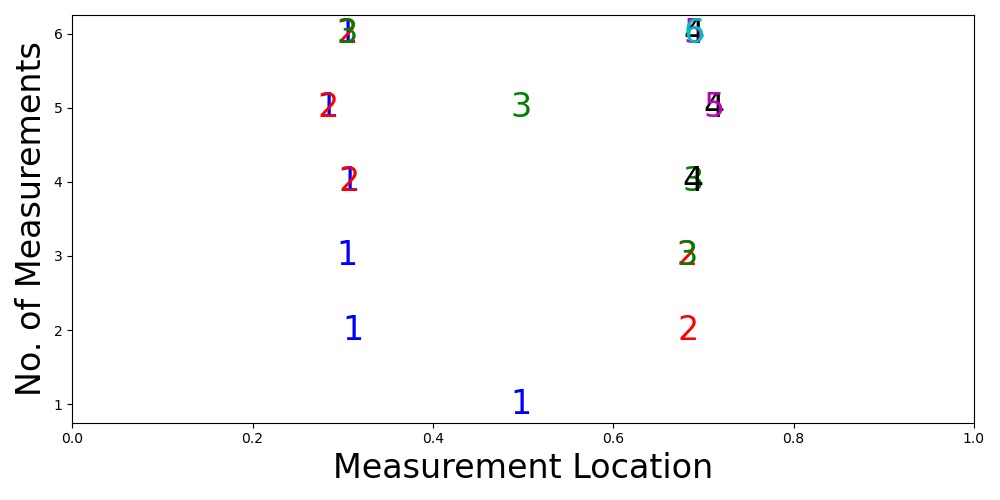
\includegraphics[height=0.5\textwidth]{figs/dst_modelError0.png}
    \caption{Measurement clusterization in D-optimal designs for the
      inverse problem of the 1D heat equation. Measurement locations
      were chosen according to the Bayesian D-optimality criterion of
      Theorem \ref{thm:d_optimality}. Measurement locations are
      plotted over the computational domain \(\Omega = [0, 1]\)
      (x-axis), for varying numbers of measurements (y-axis). The
      colored numbers are measurement indices, plotted for visual
      clarity. Measurement clusterization already occurs for three
      measurements: the second measurement (red) is overlaid on the
      third (green). For five measurements, first (blue) and second
      (red) measurements are clustered, as well as the fourth (black)
      and the fifth (magenta).}
  \label{fig:clusterization_illustration}
\end{figure}


%% Replication 1
Clusterization should not be confused with replication. Replication
requires that the experimentalist executes multiple trials under
circumstances that are \emph{nominally identical} \cite[Section
  1.2.4]{morris2011}. Replication is commonly viewed as a beneficial
and even necessary aspect of optimal experimental design
\cite{fisher1949design, morris2011, schafer2001replication}.
For example, \cite{fisher1949design}, suggested repeating his famous
milk and tea experiment in order "to be able to demonstrate the
predominance of correct classifications in spite of occasional
errors". Unfortunately, in the experiments we consider, replication is
impossible. For example, in the MRI problem, we cannot generate an
individual nominally identical to the one we wish to scan.

Similarly to a design implementing replication, a clustered design
reduces the signal-to-noise ratio of the repeated measurements
\cite{telford2007brief}. The difference is that a clustered design
takes repeated measurements at the expense of other quantities not
measured at all. For example, consider an experiment measuring the
effect of rainfall on grass growth \cite{fay2000rainfall}. The
experiment involved four rainfall manipulation "treatments"
(i.e.~simulating different timing and quantity of rainfall), each
replicated three times over different plots of land. Indeed, it seems
reasonable for researchers to replicate the phenomenon they are trying
to study. A clustered design in such an experiment would imply the
researchers should take a repeated measurement \emph{on the same
plot}, at the expense of measuring grass growth in other plots!

To conclude our short discussion on replication vs.~clusterization:
these are fundamentally different concepts and even though replication
is quite intuitive, it is inapplicable to the inverse problems we
consider in this manuscript.

Researchers of inverse problems widely agree that measurement
clusterization is undesirable \cite{fedorov1996, nyberg2012,
  fedorov1997, Ucinski05, neitzel2019sparse}, prompting the
exploration of various remedies to address this issue. One approach
involves merging close measurements \cite{fedorov1997}; however, this
strategy merely overlooks the phenomenon of measurement
clusterization. An alternative solution lies in
\emph{clusterization-free design}s, where measurement locations are
deliberately chosen to be distant from one another. This can be
achieved by imposing distance constraints between measurements or by
introducing correlated errors that account for both observation error
and model misspecification \cite{Ucinski05}. For instance, in the
context of time-series analysis for pharmacokinetic experiments,
measurement clusterization can be mitigated by incorporating the
modeling of auto-correlation time within the noise terms
\cite{nyberg2012}.


In spatial problems involving choice of measurements within a domain
\(\Omega \subseteq \mathbb{R}^d, d=1,2,3\), many researchers
circumvent the problem of measurement clusterization by restricting
measurements to a coarse grid in \(\Omega\) \cite{koval2020,
  alexanderian2021, attia2022, alexanderian2014, alexanderian2016,
  alexanderian2018efficient, brunton2016}. This approach incurs a
significant computational cost as it requires solving a difficult
combinatorial optimization problem for measurement locations over a
discrete set. The combinatorial optimization problem is usually
relaxed by first assigning optimal measurement weights in
\(\mathbb{R}_+\) to the potential measurement locations. Some
researchers incorporate a sparsifying \(\ell_1\) penalty term into the
design criterion, which is subsequently thresholded to achieve the
desired binary design over the coarse grid
\cite{horesh2008borehole}. Others progressively relax the \(\ell_1\)
penalty to an \(\ell_0\) penalty via a continuation method
\cite{alexanderian2016, alexanderian2014}. Others cast the problem of
finding optimal measurement weights as a stochastic optimization
problem \cite{attia2022stochastic}. All of the aforementioned methods
may indeed find a binary optimal design restricted to a given coarse
grid. However, none addresses one fundamental issue: the restriction
of measurement locations to a coarse grid in \(\Omega\) fundamentally
changes the optimal design problem and thus results in a sub-optimal
design.

Avoiding measurement clusterization is a pragmatic approach:
intuitively, researchers recognize that measurement clusterization is
undesirable, even though the underlying reasons may not be fully
clear. Consequently, they strive to prevent it and devise various
methodologies to avoid it. Yet each and every one of these
methodologies achieves its objective by imposing restrictions on
measurement locations, thereby fundamentally altering the optimal
design problem. To the best of my knowledge, no previous study has
tried to address some seemingly simple yet fundamental questions:
%
Why does imposing correlations between observations alleviate
measurement clusterization?
%
Is measurement clusterization a generic phenomenon? 
%
And, most importantly: Why does measurement clusterization occur?
%
%Should we aim to avoid measurement clusterization?
%
%Is it possible to substitute an optimal clustered design with an
%equally optimal non-clustered design?
%Can an optimal clustered design be replaced with an equally optimal
%non-clustered design?


\subsection{Contribution}
The primary objective of this study is to provide a deep understanding
of measurement clusterization by addressing the aforementioned
questions. Our focus centers around investigating the Bayesian
D-optimality criterion. We conduct an analysis of Bayesian D-optimal
designs within the context of linear inverse problems over Hilbert
spaces and study two inverse problems: (a) In Sections
\ref{section:prelim} and \ref{section:D_and_grad} we propose a novel
generic model for an inverse problem where D-optimality maintains
analytical tractability and D-optimal designs are identified via
Lagrange multipliers. This analytical framework facilitates the
exploration of the questions posed at the end of the previous
paragraph. We also study (b) the inverse problem of the 1D heat
equation from Section \ref{subsec:toy} above. Investigating both
inverse problems allows us to answer the questions posed in the
previous section:

\begin{enumerate}
\item \label{q:generic} \textbf{Is measurement clusterization a
  generic phenomenon?}
  %\subsection{An answer for Question \ref{q:generic}: Genericity of measurement clusterization}
  %% Computer implementation of Lemma \ref{thm:char} for the inverse
  %% problem outlined in Section \ref{section:how} also generates \(\obs\)
  %% as a solution to the D-optimal design problem.  Furthermore,
  We give two complementing answers to this question. First, from a
  theoretical perspective, we show that clusterization mainly depends
  on how quickly the eigenvalues of the prior covariance in
  observation space decay.
  %% This decay depends mostly on how ill-posed the problem at hand is
  %% and does not depend much on the prior
  See Section \ref{section:vanishing} --- particularly, Theorem
  \ref{thm:char} and the discussion following it. Furthermore, in
  Section \ref{subsec:lemma_sims} we show results of numerical
  experiments, where simulations of our model give rise to D-optimal
  designs that exhibit clusterization with high probability. Thus,
  given the genericity of our model, we expect measurement
  clusterization to be a generic and ubiquitous phenomenon.

\item \label{q:mitigate} \textbf{Why does imposing correlations
  between observations alleviate measurement clusterization?} In
  Section \ref{section:non_vanishing}, we rigorously demonstrate the
  role of model error in mitigating clusterization, thereby
  corroborating earlier observations made by various
  researchers. Specifically, our proof shows that identical
  measurements result in no gain in design criterion when observation
  error amplitude tends to zero. Moreover, in Section
  \ref{subsec:corr_errors_sims}, we show that an error term
  corresponding to correlations between measurements mitigates
  clusterization in the inverse problem of the 1D heat equation.

\item \label{q:why} \textbf{Why does measurement clusterization
  occur?} In Sections \ref{subsec:why} we give two compelling answers
  to this question by (i) transporting insights we gain from our
  generic model to the inverse problem of the 1D heat equation, and
  (ii) connecting measurement clusterization to Carath\'eodory's
  Theorem.

  Our analysis for the heat equation relies on conclusions from our
  generic model. In particular, Theorem \ref{thm:char} reveals that a
  D-optimal design focuses on a select set of prior eigenvectors,
  i.e.~those with the largest eigenvalues in the prior covariance
  spectrum. In practical scenarios, the number of locations where (a)
  all relevant prior eigenvectors are significantly large, and (b)
  other eigenvectors are close to zero, is limited. Consequently, the
  clusterization of measurements arises as a natural consequence of
  the pigeonhole principle, as there are more measurements available
  than there are locations satisfying conditions (a) and (b).

  The connection to Carath\'eodory's Theorem also builds on the focus
  of measurement effort to the abovementioned select set of prior
  eigenvectors. This allows us to move from an infinite-dimensional
  setting to finite dimensions, where the conditions of
  Carath\'eodory's Theorem hold. We conclude that a D-optimal design
  arises by weighting a small number of measurements. If the number of
  allowed measurements is larger than the small number dictated by
  Carath\'eodory's Theorem, we have excessive weight on some
  measurements, which can be interpreted as clusterization.
  
\end{enumerate}

\subsubsection{Implications}\label{subsub:implications}
Our answer to Question \ref{q:generic} implies that encountering
clusterization could be expected in many different problems across
many different scientific fields. Researchers that encounter
clusterization should not be surprised or wary. In Our answer to
Question \ref{q:why}, we explain what our view of the cause of
clusterization is. It appears, the cause is generic: a D-optimal
design reduces uncertainty for a select set of prior covariance
eigenvectors --- those with the most prior uncertainty, i.e.~those the
practitioner cares about the most!

A further implication of the analysis we present is that
clusterization can serve as an evidence to the number of relevant
eigenvectors in the problem. These eigenvectors correspond to the
relevant degrees of freedom in the problem. Thus, clusterization tells
us that we might be able to reduce the complexity of a computational
model, e.g.~by dropping discretization points.

%% Gaussian
One potential cause of clusterization is our choice of prior. Gaussian
priors, coupled with a Gaussian likelihood and a linear forward
problem give rise to a closed form solution for the posterior via
conjugacy. As we show in Section \ref{subsec:lemma_sims}, such
assumptions generically give rise to clusterization. While an
assumption of a Gaussian likelihood is standard, and rooted in the
central limit theorem, an assumption of Gaussian prior is merely a
matter of convenience. Therefore, we advise any practitioner who
encounters clusterization to replace their Gaussian priors with
non-Gaussian priors instead \cite{hosseini2017, hosseini2019}.

%% Linearization
Another potential cause of clusterization is linearization. While in a
real applications the model is not necessarily linear, some authors
consider a linearized version of their model when seeking optimal
designs \cite{fedorov1996, neitzel2019sparse}. Our analysis then shows
that the linearity of the forward problem is also an important
ingredient in giving rise to clustered designs. Therefore, our advice
to practitioners is to avoid linearization, and find D-optimal designs
via other methods, e.g.~the sampling method of \cite{ryan2003}.

%% Avoid
Given the above discussion, it is our belief that the methods
suggested by other authors to avoid clusterization are merely
overlooking the problem. We do not view clustered designs as
inherently bad on their own. Rather, we suggest that if a clustered
design arises, a practitioner should revisit their modeling choices
--- specifically, their choice of prior and model linearization. If
the practitioner is confident in their analysis, then clustered
designs should be avoided only to the extent necessitated by the
physical measuring apparatus.

%% Convergence
Clusterization in D-optimal designs raises the question of whether
D-optimal designs should be pursued at all. While other authors have
established convergence results for decaying measurement error
\cite{knapik2011}, space-filling measurements \cite{teckentrup2020}
and randomly sampled designs \cite{nickl2023}, their results do not
hold for D-optimal designs. Luckily, we can expect convergence from
D-optimal designs (including clustered designs) in the following
sense: the posterior uncertainty ellipsoid will contract to zero along
each one of its eigenvectors. See Section \ref{subsub:convergence} for
a precise statement and a proof based on Theorem \ref{thm:char} ---
the main theorem of this manuscript.


\subsubsection{Other Contributions}
In Theorem \ref{thm:char}, we also show that D-optimal designs are
best understood in the space of \emph{observations}
%% , see Section \ref{section:vanishing} for a precise statement.
This is in accordance with previous work by \cite{koval2020}, who
showed that A-optimal designs are best constructed in the space of
observations.

In the process of proving Theorem \ref{thm:char} we prove and
generalize several lemmas. Among those, is Lemma \ref{lemma:free},
which is (to the the best of my knowledge) novel: We decompose a
symmetric positive definite matrix \(M \in \mathbb{R}^{k \times k}\)
with \(\ttr M = m \in \mathbb{N}\) as \(M = AA^t\), where \(A\in
\mathbb{R}^{k \times m}\) has unit norm columns.


\subsection{Limitations}\label{subsec:limitations}
The main limitation of this study is that our generic model does not
correspond to any specific real-life problem. Specifically, in its
current form, our model does not allow point evaluations. Thus, while
our model is generic enough to be analytically tractable, one may
argue that our model is too far removed from any real application. To
these claims I would answer that scientists have a long history of
studying models that are bare-bones simplifications of real systems,
e.g.~the Ising model \cite{cipra1987}, the Lorenz system \cite{brin},
the Lotka-Volterra equations \cite{logan2006}, the Carnot engine
\cite{kardar2007} and many others.




































%% When clusterization arises, we believe it should serve as a warning
%% signal to practitioners. In the inverse problem of the 1D heat
%% equation, clusterization occurs primarily because Laplacian
%% eigenvectors do not decay in $\Omega$. Consequently, measuring $u(x_1,
%% T)$ at some point $x_1 \in \Omega$ provides information about
%% $u(x_2,T)$ for distant points $x_2 \in \Omega$. Intuitively, this
%% should not happen: for small $T$, the heat distribution at $x_1$
%% should give very little knowledge on the heat distribution at
%% $x_2$. This behavior stems from a well-known property of the heat
%% equation: it allows information to spread instantly across the
%% computational domain \cite{renardy2006PDE}. In reality, heat (and
%% information) propagate at finite speeds. Of course, the known physical
%% barrier for information spread is the speed of light, but we expect
%% heat and information to spread considerably slower. Thus,
%% clusterization may suggest that our physical model itself is at fault.

%% We believe that the emergence of clusterization in this context might
%% be non-physical, arising from the way the inverse problems we consider
%% are phrased. Clusterization therefore indicates that the underlying
%% mathematical / Bayesian model is overly permissive and fails to
%% capture crucial physical constraints of the problem. We suggest that
%% when clusterization occurs, practitioners should consider alternative
%% models where information is localized in space and travels at finite
%% speed in the medium. Such models may not only provide more physically
%% accurate and meaningful results but may also mitigate the issue of
%% clusterization.



%% be avoided at all. Nothing in our analysis indicates that we should
%% expect any pathological behavior when utilizing D-optimal designs. On
%% the contrary: we show that D-optimal designs (clustered or not) reduce
%% uncertainty of prior covariance eigenvectors where it is
%% highest. Thus, in a sense we hope to make precise in a future study,
%% we expect convergence of for D-optimal designs to be fastest.



%% practitioners should not try to avoid measurement
%% clusterization. Rather, practitioners should take repeated
%% measurements (e.g.~in MRI and borehole tomography), increase apparatus
%% sensitivity (e.g.~in EIT), or take consecutive measurements (e.g.~in
%% the 1D heat equation). Overall, we show that measurement
%% clusterization is a natural and (almost) inevitable part of Bayesian
%% D-optimal designs (but see disclaimer below).

